\section{Theoretical Overview}
Pathfinding in modern video games often involves exploring highly regular 
\label{algorithm}
environments such as cities, sewers or dungeons.
These locales tend to be topographically simple and frequently comprise only
empty rooms and corridors between them.
As we showed in Figure \ref{fig-emptymap} however it is exactly these 
types of environments which A* has the most difficulty with.
The main difficulty facing A* is that all nodes in an empty or near 
empty room have very similar or even identical f-costs.
To preserve optimality A* must expand all such nodes until it can prove they do 
not appear on the optimal path.
%Figure \ref{fig-oha_contrast}(a) illustrates such a case; 
%notice that A* explores almost half the map. 
\par
To overcome these difficulties we propose the following simple search strategy:
instead of exploring the interior of an empty room expand only nodes along the
perimeter. We claim that this approach preserves optimality when searching in 
4-connected grid maps. 
Consider the following argument:

\begin{mylemma}
\label{thm-roomtraversal}
For every optimal length path segment running through the interior of an empty 
4-connected rectangular room $R$ there exists another equivalent length path 
segment which involves only nodes from the perimeter of $R$.
\end{mylemma}
\begin{proof}
Let $s, g \in R$ correspond to the endpoints of an optimal length path segment 
$\pi(s, g)$ running through R.
There are three cases we need to consider depending on whether the segment 
is at the beginning, middle or end of some long optimal path that crosses
many rooms.
\par
First, suppose $\pi(s, g)$ is the segment at the end of the optimal path.
Then $g$ is the final goal node and, in all likelihood, is located in the 
interior of $R$ (as per Figure \ref{fig-roomtraversal}(a)).
In this case we can simply use a manhattan heuristic to exactly calculate $h^*(s, g)$.
Since $R$ is empty the heuristic is perfectly informed and we may generate $g$
as a direct \emph{macro successor} of $s$ without expanding any nodes from the interior of $R$.
\par
Next, suppose $\pi(s, g)$ is the segment at the beginning of the optimal path. 
Then, $s$ is, in all likelihood, located in the interior of $R$ 
(as per Figure \ref{fig-roomtraversal}(b)) while $g$ is located on the perimeter.
In this case we proceed by expanding $s$ to generate the macro successor set 
$\Gamma(s) = \lbrace s_{1}', s_{2}', s_{3}', s_{4}'\rbrace$.
Each $s_{i}'$ is the closest perimeter node to $s$ along each of the four sides of $R$.
Since $h^*$ is perfectly informed the cost of each macro edge 
$c(s, s_{i}') = h^*(s, s_{i}')$ is optimal.
Further, since $g$ is on the perimeter of $R$, there must exist a path $\pi(s_{i}', g)$ 
such that the cost of $\pi(s, g) = \pi(s, s_{i}') + \pi(s_{i}', g)$ is optimal.
To see that this is true simply choose the $s_{i}'$ closest to $g$.
It follows that since $\pi(s, min(s_{i}'))$ is optimal and $\pi(min(s_{i}', g)$
is optimal it must be that $\pi(s, g)$ is also optimal. 
\par
Finally, suppose that $\pi(s, g)$ is a segment in the middle of the optimal path.
Then, $s$ and $g$ are both located on the perimeter of $R$ 
(as in Figure \ref{fig-roomtraversal}(c)). 
If $g$ is on the same side of the perimeter to $s$ or on one of the two orthogonal sides 
it follows that we can find an optimal length path between them by the successive expansion of 
nodes adjacent to $s$ along the perimeter.
Suppose however that $g$ is somewhere on the opposide side of $R$.
In this case we can generate a single macro successor $s'$ which appears on the 
perimeter of $R$ directly opposite to $s$.
It now becomes trivial to show that there exists a minimum lengh path $\pi(s',g)$.
Further, since $h^*$ is perfectly informed, the cost of $\pi(s, s')$ is also optimal
which means that $\pi(s, g) = \pi(s, s') + \pi(s', g)$ must be optimal.
\end{proof}

\begin{figure}[htbp]
	\label{fig-roomtraversal}
	\vspace{-4pt}
       \begin{center}
           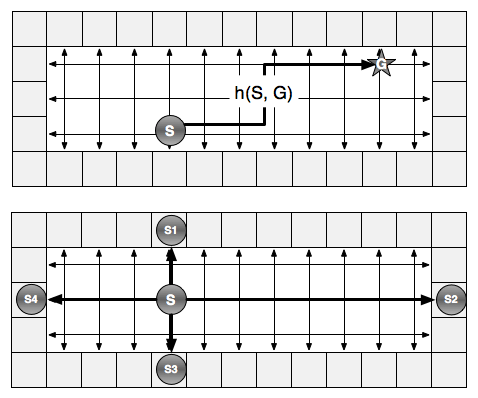
\includegraphics[scale=0.50, trim = 10mm 10mm 10mm 0mm]{diagrams/roomtraversal.png}
       \end{center}
	\vspace{-3pt}
       \caption{The three cases which must be considered in order to prove that 
			optimal traversal of an empty room is possible using only nodes from the perimeter.
			Dashed lines represent macro successors and solid lines represent segments of optimal
			paths that are eventually found}
       \label{fig-ohacontrast}
	\vspace{-15pt}
\end{figure}

A direct corrolary Lemma \ref{thm-roomtraversal} is that we can prune from consideration
all nodes from the interior of $R$ and limit ourselves to those nodes appearing along its perimeter.
In light of this result we propose the following hierarchical search strategy for finding shortest 
paths in 4-connected grid maps:

\begin{enumerate}
\item{\label{oha-step1} Preprocess a 4-connected grid map in order to construct a set of adjacent empty rooms such that 
each room is rectangular in shape and each tile on the map is assigned to exactly one room. }
\item{\label{oha-step2} Begin the search by expanding the start node as described in 
Lemma \ref{thm-roomtraversal} in order to generate the set 
$\Gamma(s) = \lbrace s_{1}', s_{2}', s_{3}', s_{4}'\rbrace$ which are added to the open list. }
\item{\label{oha-step3} Using any graph search algorithm evaluate the set of open nodes.}
\item{\label{oha-step4} When expanding a node $x$ that is not in the goal room generate the set 
$\Gamma(x) = \lbrace p, q, x' \rbrace$ as described in Lemma \ref{thm-roomtraversal} and updating the open
list as required.} 
\item{\label{oha-step5} When expanding a node $s$ that is in the goal room generate $g$ directly as 
described in Lemma \ref{thm-roomtraversal}} 
\item{Repeat steps \ref{oha-step3}-\ref{oha-step5} until either the goal is found (in which case return
the path) or all nodes have been evaluated (in which case return failure).}
\end{enumerate}
When the graph search algorithm at step \ref{oha-step3} is A* we term the resulting algorithm 
Optimal Hierarchical A* (or simply OHA*).

\begin{figure*}[htbp]
	\label{fig-oha_contrast}
	\vspace{-4pt}
       \begin{center}
           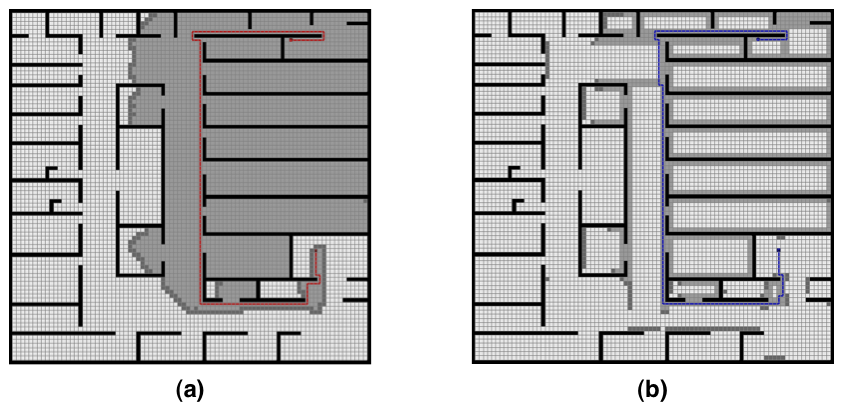
\includegraphics[scale=0.60, trim = 10mm 10mm 10mm 0mm]{diagrams/oha_contrast.png}
       \end{center}
	\vspace{-3pt}
       \caption{\textbf{(a)} A* solving a problem on a typical ($86\times88$) game map. 
Expanded nodes are marked light grey while nodes at the frontier of the search are dark grey.
\textbf{(b)} OHA* solving the same problem. A number of large rooms have been identified (not
all shown) and the algorithm only considers nodes along their perimeter.}
       \label{fig-ohacontrast}
	\vspace{-15pt}
\end{figure*}


\begin{mytheorem}
OHA* is optimal. 
\end{mytheorem}
\begin{proof}
To prove this claim we have to show that for every optimal length path $\pi^*(m, n)$ 
on a 4-connected grid map, which starts at node $m$ and terminates at node $n$, 
there exists an equivalent length path $\pi^{*'}(m, n)$ that mentions only nodes from the
perimeter of $R$.
The proof is almost immediate following Lemma \ref{thm-roomtraversal}. 
We will show it is true using an structural proof by induction on the length
of $\pi^{*'}(m, n)$.
\par
For the basis case, suppose node $m$ and $n$ are in the same room $R$.
In this case the optimal $g-costs$ of $m$ and $n$ are given by:
$$g^*(m) = 0$$
$$ g^*(n) =  \sum_{i = m}^{p(n)}c(k_{i}, k_{i+1})$$ 

where $p(n)$ is the node that preceeds $n$ on the optimal path and $c$ is the cost of 
an edge connecting nodes $k_{i}$ and $k_{i+1}$ which appear in sequence along the optimal path 
and are both ancestors of $n$.
We construct $\pi'(m, n)$ by way of Lemma \ref{thm-roomtraversal}, 
which states that we can use the heuristic function $h^*$ to directly generate $m$ as a 
macro successor of $n$ if both are in the same room.
Thus we have:

$$ g^{*'}(m) = 0 $$
$$ g^{*'}(n) = h^*(m, n)$$

To see that these are equivalent we may restate $g^*(n)$ as:
$$g^*(n) = |x_{m} - x_{n}| + |y_{m} - y_{n}| = h^*(m, n)$$

where $x_{m}, y_{m}$ are the coordinates of node $m$ on the map and $x_{n}, y_{n}$ are
the coordinates of node $n$.
We can calculate $g(n)$ in this fashion only because $\pi^*(m,n)$ is optimal and $R$ is
obstacle free which eliminates the possibility that the optimal path contains
 switchbacks (segments where the path doubles back on itself).
Thus $g^{*}(m) = g^{*'}(m)$.
\par
For the inductive case we must show that the same analysis which was true for the basis case
is also true for any segment of the optimal path running through some room $R$. 
Lemma \ref{thm-roomtraversal} gives just such an analysis.
Since every segment of $\pi^{*}(m, n)$ has a corresponding segment in $\pi^{*'}$ of equivalent
length it must be that $g^*(n) = g^{*'}(n)$ and $g^*(m) = g^{*'}(m)$.
\end{proof}

To highlight how well OHA* can work in practice consider the example game map in Figure 
\ref{fig-oha_contrast}. 
The topography of this map is typical of what one might expect in a modern roleplaying game
\footnote{Infact, most video game maps tend to be somewhat bigger than our example but for demonstration 
purposes it is quite sufficient.};
there are many rooms and corridors and many entrances to connect them.
In Figure \ref{fig-oha_contrast}(a) we show A* solving a typical problem on this map. 
In this case obtaining the optimal solution required expanding almost half the nodes on the map.
Figure \ref{fig-oha_contrast}(b) shows the same problem being solved by OHA*.
We were able to prune away large sections of the map by taking advantage of the fact that
such nodes never need to be expanded in order to retain optimality.
In this case OHA* expands less than $\frac{1}{3}$ of the area explored by A* and returns
a solution 4 times faster.

